\documentclass[a4paper,12pt]{article}
\usepackage{cmap}
\usepackage[utf8]{inputenc}
\usepackage[warn]{mathtext}
\usepackage{epsf,amsmath,amsfonts,amssymb,amsbsy}
\usepackage[mathscr]{eucal}
\usepackage[english, russian]{babel}
\author{Мещеряков Павел Б02-920}
\title{Отчёт о выполнении лабораторной работы 2.1.3}
\usepackage[left=2cm,right=2cm,top=2cm,bottom=2cm]{geometry}
\usepackage{graphicx}
\usepackage{indentfirst}
\graphicspath{{pictures2.1.3/}}
\DeclareGraphicsExtensions{.pdf,.png,.jpg}
\usepackage{pgfplots}
\begin{document}
	\maketitle
	\begin{center}
		{\Large Определение $C_p/C_v$ по скорости звука в газе}
	\end{center}
	\paragraph*{Цель работы:} 1) измерение частоты
	колебаний
	и длины волны при
	резонансе звуковых
	колебаний в газе, заполняющем трубу; 2) определение показателя адиабаты с помощью уравнения состояния идеального газа.
	\paragraph*{В работе используются:} звуковой генератор ГЗ; электронный
	осциллограф ЭО; микрофон; телефон; раздвижная труба; теплоизолированная труба, обогреваемая водой из термостата; баллон
	со сжатым углекислым газом; газгольдер.
	\section{Теоретическое введение}
	
		Cкорость распространения звуковой волны в газах зависит от показателя адиабаты $\gamma$. На измерении скорости звука основан один из наиболее  точных методов определения показателя  адиабаты.
		
		Скорость звука в газах определяется формулой:
		$$c=\sqrt{\gamma\frac{RT}{\mu}},$$
		где $R$ - газовая постоянная, $T$ - температура газа, а $\mu$ его молярная масса. Выразим показатель адиабаты:
		$$\gamma=\frac{\mu}{RT} c^2$$
		
		Звуковая волна, распространяющаяся вдоль трубы, испытывает многократные отражения от торцов. Звуковые колебания в трубе являются наложением всех отраженных волн и, вообще говоря, очень сложны. Картина упрощается, если длина трубы L равна целому числу полуволн, то есть когда
		$$L=n\frac{\lambda}{2},$$
		где $\lambda$ — длина волны звука в трубе, а $n$ — любое целое число.
		
		Скорость звука c связана с его частотой $f$ и длиной волны $\lambda$ соотношением:
		$$c=\lambda f.$$
		
		Подбор условий, при которых возникает резонанс, можно производить двояко:
		
		1) При неизменной частоте f звукового генератора (а следовательно, и неизменной длине звуковой волны $\lambda$) можно изменять длину трубы $L$. Для этого применяется раздвижная труба. Длина раздвижной трубы постепенно увеличивается, и наблюдается ряд последовательных резонансов. Для $k$-ого резонанса имеем:
		$$L_{n+k}=n\frac{\lambda}{2} + k\frac{\lambda}{2},$$
		т. е. $\lambda/2$ равно угловому коэффициенту графика, изображающего зависимость длины трубы $L$ от номера резонанса $k$.
		
		2) При постоянной длине трубы можно изменять частоту звуковых
		колебаний. В этом случае следует плавно изменять частоту $f$ звукового генератора, а следовательно, и длину звуковой волны $\lambda$.
		Для $k$-ого резонанса получим:
		$$L = (n+k)\frac{\lambda_{k+1}}{2}$$
		$$f_{k+1} = \frac{c}{\lambda_{k+1}}=\frac{c}{2L}(n+k)=f_1 + \frac{c}{2L}k.$$
		
		Скорость звука, деленная на $2L$, определяется, таким образом,
		по угловому коэффициенту графика зависимости частоты от номера
		резонанса.
	\subsection{Эксперементальная установка:}
	\begin{figure}[h]
	\center{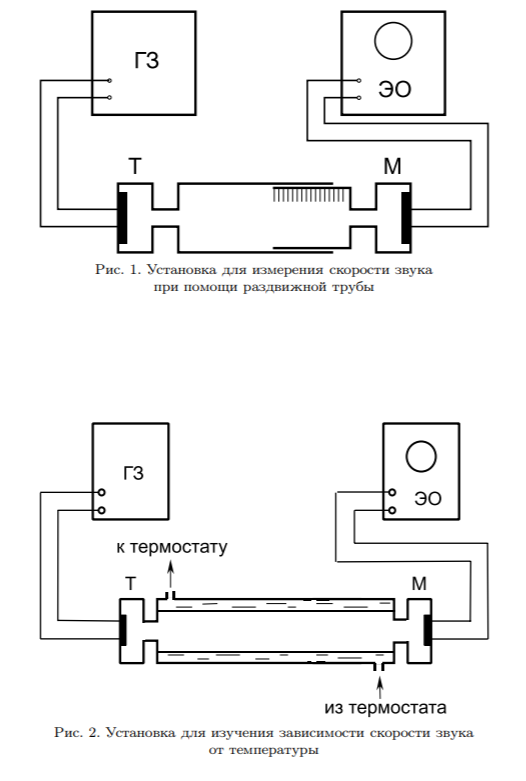
\includegraphics[scale=0.65]{lab_2_1_3_ust}}
	\end{figure}
	Соответственно двум методам измерения скорости звука в работе имеются две установки (рис. 1 и 2). В обеих установках звуковые колебания в трубе возбуждаются телефоном Т и улавливаются микрофоном М. Мембрана телефона приводится в движение переменным током звуковой частоты; в качестве источника переменной ЭДС используется звуковой генератор ГЗ. Возникающий в микрофоне сигнал наблюдается на осциллографе ЭО.

	Микрофон и телефон присоединены к установке через тонкие резиновые трубки. Такая связь достаточна для возбуждения и обнаружения звуковых колебаний в трубе и в то же время мало возмущает эти колебания: при расчетах оба торца трубы можно считать неподвижными, а влиянием соединительных отверстий пренебречь.

	Первая установка (рис. 1) содержит раздвижную трубу с миллиметровой шкалой. Через патрубок (на рисунке не показан) труба может наполняться воздухом или углекислым газом из газгольдера. На этой установке производятся измерения $\gamma$ для воздуха и для $CO_2$.
	
	Вторая установка (рис. 2) содержит теплоизолированную трубу постоянной длины. Воздух в трубе нагревается водой из термостата. Температура газа принимается равной температуре омывающей трубу воды. На этой установке измеряется зависимость скорости звука от температуры.

	\subsection{Ход работы}
	\begin{enumerate}
		\item Перепишем параметры установки:
		$L = 700\pm1 \; {мм}.$
		\item  
		
		Исходя из примерного значения скорости звука ($ \approx 270 \; \frac{м}{с}$), предварительно рассчитаем, в каком диапазоне частот следует вести измерения, чтобы при удлинении трубы можно было наблюдать 4 резонанса:
$L = \frac{n\lambda}{2}$, $L + \Delta L = \frac{(n+4)\lambda}{2}$. Поскольку $\Delta L \leq 23 \; {см}$, то $\lambda \leq 11.5 \; {см}$. Следовательно $f \geq 2400 \; {гц}. $
		
		Проведём измерения на первой установке для $CO_2$.
		Плавно изменяя длину трубы, последовательно зафиксируем все доступные для наблюдения точки резонанса. Измерения проводятся для нескольких частот.
		\begin{center}
		\begin{tabular}{|l|l|l|l|l|l|l|l|l|l|}
			\hline
			f, Гц & \multicolumn{2}{|c|}{2492} & \multicolumn{2}{|c|}{2751}&  \multicolumn{2}{|c|}{3016} & \multicolumn{2}{|c|}{3265}
			\\
			\hline
			k &  $l_1$, см& $l_2$, см & $l_1$, см & $l_2$, см & $l_1$, см & $l_2$, см & $l_1$, см & $l_2$, см
			\\
			
			\hline
			0 & 0 & 0 & 0.2 & 0.2 & 0.9 & 0.9 & 1.0 & 1.0
			\\
			\hline
			1 & 5.0 & 5.8 & 6.0 & 6.0 & 6.2 &  6.1 & 5.5 & 5.3
			\\
			\hline
			2 & 11.0 & 10.8 & 10.5 & 10.3 & 11.5 & 11.5 & 9.7 & 9.4
			\\
			\hline
			3 & 17.0 & 17.1 & 16.0 & 15.5 & 17.2 & 17.2 & 11.4 & 11.5
			\\
			\hline
			4 & 23.0 & 22.9 & 19.5 & 20.0 & 22.5 & 22.5 & 18.8 & 18.5
			\\
			\hline
		\end{tabular}
		\end{center}
		$l_1$ соответсвует значение на размеченной подвижной части трубы укорачиванию длины, а $l_2$ удлинению.
		\item Изобразим полученные результаты на графике, откладывая по оси абсцисс номер $k$ последовательного резонанса, а по оси ординат — соответствующее удлинение трубы
		$\Delta l$. Угловой коэффициент прямой определяет длину полуволны.
		
\begin{center}
	\begin{tabular}{lr}
			\begin{tikzpicture}[scale = 0.8]
			\begin{axis}[
			axis lines = left,
			legend style={at={(1,0.3)}},
			xlabel = {$k$},
			ylabel = {$\Delta l, {см} $
			},
			xmin=0, xmax=5,
			ymin=0, ymax=24,
			ymajorgrids = true,
			xmajorgrids = true,
			minor tick num = 4
			]
			\addplot+[only marks ] plot[error bars/.cd, y dir=both, y explicit]
			coordinates {
				(0,0) +- (0.1,0.1)
				(1, 5) +- (0.1,0.1)
				(2, 11) +- (0.1,0.1)
				(3, 17) +- (0.1,0.1)
				(4, 23) +- (0.1,0.1)
				(0,0) +- (0.1,0.1)
				(1, 5.8) +- (0.1,0.1)
				(2, 10.8) +- (0.1,0.1)
				(3, 17.1) +- (0.1,0.1)
				(4, 22.9) +- (0.1,0.1)
			};
			\addplot[red, domain=0:4.5] {-0.25+5.755*x};
			
			\legend{
				$$f = 2492 {Гц}, y = -0.25+5.755x$$
			};
 			\end{axis}
			\end{tikzpicture}	
			&
			
			\begin{tikzpicture}[scale = 0.8]
			\begin{axis}[
			axis lines = left,
			legend style={at={(1,0.3)}},
			xlabel = {$k$},
			ylabel = {$\Delta l, {см} $
			},
			xmin=0, xmax=5,
			ymin=0, ymax=24,
			ymajorgrids = true,
			xmajorgrids = true,
			minor tick num = 4
			]
			\addplot+[only marks ] plot[error bars/.cd, y dir=both, y explicit]
			coordinates {
				(0,0) +- (0.1,0.1)
				(1, 5.8) +- (0.1,0.1)
				(2, 10.3) +- (0.1,0.1)
				(3, 15.8) +- (0.1,0.1)
				(4, 19.8) +- (0.1,0.1)
				(0,0) +- (0.1,0.1)
				(1, 5.8) +- (0.1,0.1)
				(2, 10.1) +- (0.1,0.1)
				(3, 15.3) +- (0.1,0.1)
				(4, 19.8)	+- (0.1,0.1)
			};
			\addplot [red, domain=0:4.5]{0.45+4.885*x};
			
			\legend{
				$$f = 2751{Гц},y=0.45+4.885x$$
			};
						\end{axis}
			\end{tikzpicture}
			\\	
			
			\begin{tikzpicture}[scale = 0.8]
			\begin{axis}[
			axis lines = left,
			legend style={at={(1,0.3)}},
			xlabel = {$k$},
			ylabel = {$\Delta l, {см} $
			},
			xmin=0, xmax=5,
			ymin=0, ymax=24,
			ymajorgrids = true,
			xmajorgrids = true,
			minor tick num = 4
			]
			
			\addplot+[only marks ] plot[error bars/.cd, y dir=both, y explicit]
			coordinates {
				(0,0) +- (0.1,0.1)
				(1, 5.3) +- (0.1,0.1)
				(2, 10.6) +- (0.1,0.1)
				(3, 16.3) +- (0.1,0.1)
				(4, 21.6) +- (0.1,0.1)
				(0,0) +- (0.1,0.1)
				(1, 5.2) +- (0.1,0.1)
				(2, 12.5) +- (0.1,0.1)
				(3, 16.3) +- (0.1,0.1)
				(4, 21.6) +- (0.1,0.1)
			};
			\addplot[red, domain=0:4.5] {0.20+5.425*x};
			\legend{
				$$f = 3016 {Гц},y = 0.20+5.425x$$
			};
			\end{axis}
			\end{tikzpicture}
			
			&
			
			\begin{tikzpicture}[scale = 0.8]
			\begin{axis}[
			axis lines = left,
			legend style={at={(1,0.3)}},
			xlabel = {$k$},
			ylabel = {$\Delta l, {см} $
			},
			xmin=0, xmax=5,
			ymin=0, ymax=24,
			ymajorgrids = true,
			xmajorgrids = true,
			minor tick num = 4
			]
			
			\addplot+[only marks ] plot[error bars/.cd, y dir=both, y explicit]
			coordinates {
				(0,0) +- (0.1,0.1)
				(1, 4.5) +- (0.1,0.1)
				(2, 8.7) +- (0.1,0.1)
				(3, 10.4) +- (0.1,0.1)
				(4, 17.5) +- (0.1,0.1)
				(0,0) +- (0.1,0.1)
				(1, 4.3) +- (0.1,0.1)
				(2, 8.4) +- (0.1,0.1)
				(3, 10.5) +- (0.1,0.1)
				(4, 17.5) +- (0.1,0.1)
			};
			\addplot [red, domain=0:4.5] {-0.06+4.135*x};
			\legend{
				$$f = 3265 {Гц}, y = -0.06+4.135x$$
			};
			\end{axis}
			\end{tikzpicture}
			
			\\
	\end{tabular}
\end{center}
		
		Вычислим с помощью полученных графиков скорость звука в углекислом газе и рассчитаем погрешности.
		
		Погрешность $\sigma_{c}$ отдельного измерения определяется следующей формулой:
		$$ \sigma_{c} =c \sqrt{\Big(\frac{\sigma_{\lambda}}{\lambda}\Big)^2+ \Big(\frac{\sigma_{f}}{f}\Big)^2}.$$
		
		Результаты представлены в таблице:
		\begin{center}
		\begin{tabular}{|l|l|l|l|l|}
			\hline
			f, Гц & 2492 & 2751& 3016 & 3265
			\\
			
			\hline
			$\lambda,{м} \cdot 10^{-2} $ & 5.755 & 4.885 & 5.425 & 4.135
			\\
			\hline
			$c,\frac{м}{с}$ & 286.829 & 268.773 & 327.236 & 270.016 
			\\
			\hline
			$\sigma_{\lambda},{м} \cdot 10^{-2} $ & 0.022 & 0.022 & 0.022 & 0.022
			\\
			\hline
			$\sigma_{f},{Гц}$ & 5 & 5 & 5 & 5 
			\\
			\hline
			$\sigma_{c},\frac{м}{с}$ & 1.238 & 1.305 & 1.436 & 1.495
			\\
			\hline
		\end{tabular}
		\end{center}
		Можно заметить, что значения скоростей звука при различных частотах не совпадают.
		Усреднив полученные значения найдём окончательное значение скорости звука в углекислом газе. $$\overline{c} = 288.2 \:\frac{м}{с}$$
		$$c_{сл} = \sqrt{\frac{\sum_{i=1}^{4} (c_{i}-\overline{c})^2}{3}} = 27.2 \: \frac{м}{с}.$$
		
		$$ c_{кос} = \sqrt{\frac{\sum_{i=1}^{4} (\sigma_{c_{кос}})^2}{4^2}} = 0.69 \; \frac{м}{с}.$$
		
		Общая погрешность: $$\sigma_{c} = \sqrt{(с_{сл})^2+(c_{кос})^2} = 27.2\frac{м}{c}.$$
		Итак, $$c = 288.2 \pm 27.2 \; \frac{м}{с}.$$
		Теоретическое значение скорости при температуре $t = 24.1 ^\circ C$ равно $$с_{т} = 273.6 \: \frac{м}{с}.$$
		В пределах погрешности эксперементальное значение совпадает с теоретическим.
		Однако стоит сказать пару слов о таком сильном разбросе для $c$. Это может быть связано с тем, что подвижную часть цилиндра двигали не достаточно медленно.
		
		
		\item Проведём измерения на второй установке. Данные представлены в таблице.
		
			\begin{center}
			\begin{tabular}{|l|l|l|l|l|l|l|l|l|l|}
			\hline
			t, $^\circ C$ & \multicolumn{2}{|c|}{24.1} & \multicolumn{2}{|c|}{30}&  \multicolumn{2}{|c|}{40} & \multicolumn{2}{|c|}{50}
			\\
			\hline
			k &  $f_1$, Гц & $f_2$, Гц & $f_1$, см & $f_2$, Гц & $f_1$, Гц & $f_2$, см & $f_1$, Гц & $f_2$, Гц
			\\
			\hline
			0 & 200 & 200 & 195 & 203 & 227 & 230 & 238 & 240
			\\
			\hline
			1 & 447 & 453 & 461 & 466 & 456 & 456 & 466 & 468
			\\
			\hline
			2 & 662 & 657 & 666 & 667 & 678 & 673 & 684 & 681
			\\
			\hline
			3 & 866 & 871 & 896 & 883 & 895 &  898 & 909 & 911
			\\
			\hline
			4 & 1089 & 1089 & 1100 & 1100 & 1120 & 1120 & 1138 & 1138
			\\
			\hline
		\end{tabular}
		\end{center}
		
		$f_1$ - соотвествует значениям при увеличении частоты на трубу, $f_2$ - при уменьшении. Видно, что данные воспроизводятся при обратном ходе.		


		\item Полученные результаты изобразим на графике, откладывая
		по оси абсцисс номер резонанса $k$, а по оси ординат — разность между частотой последующих резонансов и частотой первого резонанса: $\Delta f_k = f_{k+1}-f_1.$ Угловой
		коэффициент прямой определяет величину $c/2L$.
		
\begin{center}
	\begin{tabular}{lr}
		
		\begin{tikzpicture}[scale = 0.7]
		\begin{axis}[
		axis lines = left,
		legend style={at={(1,0.3)}},
		xlabel = {$k$},
		ylabel = {$\Delta f, {Гц}$},
		xmin=0, xmax=5,
		ymin=0, ymax=1000,
		ymajorgrids = true,
		xmajorgrids = true,
		minor tick num = 4
		]
		
		\addplot+[only marks ] plot[error bars/.cd, y dir=both, y explicit]
		coordinates {
			(0,0)
			(1, 247)
			(2, 462)
			(3, 666)
			(4, 889)
			(0,0)
			(1, 253)
			(2, 457) 
			(3, 671)
			(4, 889)
		};
		\addplot[red, domain=0:4.5] {14.1 + 219.7*x};
		\legend{	
			$$ t = 24.1 { $^\circ$C}, y = 14.1 + 219.7x $$ 
		};
		\end{axis}
		\end{tikzpicture}
		&
		\begin{tikzpicture}[scale = 0.7]
		\begin{axis}[
		axis lines = left,
		legend style={at={(1,0.3)}},
		xlabel = {$k$},
		ylabel = {$\Delta f, {Гц}$},
		xmin=0, xmax=5,
		ymin=0, ymax=1000,
		ymajorgrids = true,
		xmajorgrids = true,
		minor tick num = 4
		]
		
		\addplot+[only marks ] plot[error bars/.cd, y dir=both, y explicit]
		coordinates {
			(0,0)
			(1, 266)
			(2, 471)
			(3, 701)
			(4, 905)
			(0,0)
			(1, 263)
			(2, 464) 
			(3, 680)
			(4, 897)
		};
		\addplot[red, domain=0:4.5] {19.1 + 222.8*x};
		\legend{	
			$$ t = 30 { $^\circ$C}, y = 19.1 + 222.8x $$ 
		};
		\end{axis}
		\end{tikzpicture}
		
		\\
		
		\begin{tikzpicture}[scale = 0.7]
		\begin{axis}[
		axis lines = left,
		legend style={at={(1,0.3)}},
		xlabel = {$k$},
		ylabel = {$\Delta f, {Гц}$},
		xmin=0, xmax=5,
		ymin=0, ymax=1000,
		ymajorgrids = true,
		xmajorgrids = true,
		minor tick num = 4
		]
		
		\addplot+[only marks ] plot[error bars/.cd, y dir=both, y explicit]
		coordinates {
			(0,0)
			(1, 229)
			(2, 451)
			(3, 668)
			(4, 893)
			(0,0)
			(1, 226)
			(2, 443) 
			(3, 668)
			(4, 890)
		};
		\addplot[red, domain=0:4.5] {2.1 + 222.4*x};
		\legend{	
			$$ t = 40 { $^\circ$C}, y = 2.1 + 222.4x $$ 
		};
		\end{axis}
		\end{tikzpicture}
		&
		\begin{tikzpicture}[scale = 0.7]
		\begin{axis}[
		axis lines = left,
		legend style={at={(1,0.3)}},
		xlabel = {$k$},
		ylabel = {$\Delta f, {Гц}$},
		xmin=0, xmax=5,
		ymin=0, ymax=1000,
		ymajorgrids = true,
		xmajorgrids = true,
		minor tick num = 4
		]
		
		\addplot+[only marks ] plot[error bars/.cd, y dir=both, y explicit]
		coordinates {
			(0,0)
			(1, 228)
			(2, 446)
			(3, 671)
			(4, 900)
			(0,0)
			(1, 228)
			(2, 441) 
			(3, 671)
			(4, 898)
				};
		\addplot[red, domain=0:4.5] { 224.1*x};
		\legend{	
			$$ t = 50 { $^\circ$C}, y =  224.1x $$ 
		};
		\end{axis}
		\end{tikzpicture}
	\end{tabular}
\end{center}

	Вычислим с помощью полученных графиков скорость звука в воздухе и рассчитаем погрешности. Погрешность $\sigma_{c}$ отдельного измерения определяется следующей формулой:
	$$ \sigma_{c} =c \sqrt{\Big(\frac{\sigma_{L}}{L}\Big)^2+ \Big(\frac{\sigma_{A}}{A}\Big)^2},$$
	где $A$ - коэффициент наклона прямой на графике.
	Результаты представлены в таблице:
	\begin{center}
	\begin{tabular}{|l|l|l|l|l|}
		\hline
		t, $^\circ$ C & 24.1 & 30 & 40 & 50
		\\
		
		\hline
		$A,{Гц}$ & 219.7 & 222.8 & 222.4 & 224.1
		\\
		\hline
		$c,\frac{м}{с}$ & 351.52 & 356.48 & 355.84 & 358.56
		\\
		\hline
		$\sigma_{A},{Гц} $ & 1.1 & 1.1 & 1.1 & 1.1
		\\
		\hline
		$\sigma_{L},{м} \cdot 10^{-3} $ & 1 & 1 & 1 & 1 
		\\
		\hline
		$\sigma_{c},\frac{м}{с}$ & 1.814 & 1.855 & 1.815 & 1.816
		\\
		\hline
		$\gamma$ & 1.446 & 1.458 & 1.406 & 1.384
		\\
		\hline
	\end{tabular}
	\end{center}

	По полученным данным расчитаем $\gamma$.
	$$\overline{\gamma} = 1.423$$
	$$\gamma_{сл} = \sqrt{\frac{\sum_{i=1}^{4} (\gamma_{i}-\overline{\gamma})^2}{3}} = 0.04 .$$
	Косвенная погрешность определения $\gamma$ мала, так как $\frac{2\sigma_c}{4c} \approx 0.25 \%.$
	Итак, $$\gamma = 1.42 \pm 0.04 ,$$ что в пределах погрешности совпадает  с теоретическим значением $\gamma = 1.4 .$
	Если обратить внимание на полученные значения для $c$, то можно усомниться в справедливости формулы $c^2 = \frac{\gamma R T}{\mu}$ и начать предпологать, что показатель адиабаты является функцией от температуры $\gamma = \gamma(T)$. Однако температуры в данном опыте не слишком большие и другие степени свободы не могли активироваться у молекул газа. Есть гипотеза, объясняющая такие разбросы.Вероятно измерения производились не во время достижения термодинамического равновесия и нужно было ждать приличное время (~5 минут) после того как на термостате установится необходимая температура, для того чтобы система пришла в пригодное состояние для измерений.

\end{enumerate}

\end{document}